\documentclass[12pt,oneside,a4paper]{article}
%
\usepackage{graphicx}
\usepackage{tabularx}
\usepackage{url}
\usepackage[latin1]{inputenc}
%\usepackage[utf8]{inputenc}
\usepackage[left]{eurosym} 
\usepackage{times}
\usepackage{pdfpages}
\usepackage{todonotes}
\usepackage{enumerate}

% We don't want a special font for urls (looks bad with times):
\urlstyle{same}

% Graphics extensions and path:
%\DeclareGraphicsExtensions{.pdf,.png,.jpg}
%\DeclareGraphicsExtensions{.eps,.ps}
%\graphicspath{{figures/}}

%
% Page size
%
\usepackage[top=25mm,left=25mm,right=25mm,bottom=25mm]{geometry}

\setlength{\headheight}{15pt}    % Necessary to avoid fancyhdr warning.


\newcommand\LongTitle{Humidity, clouds and snow in the Arctic}
\newcommand\ShortTitle{Humidity, clouds and snow in the Arctic}



%
% Heading
%
\newcommand{\pagevers}[2]{
\ifnum\thepage=1 
#1
\else#2
\fi
}
%
\usepackage{fancyhdr}
\pagestyle{fancy}
\chead{}
%\rhead{\pagevers{}{\bf \thepage}}
\rhead{\thepage}
\rfoot{\small \it \ShortTitle\ ---\  Application to SNSA 2021-R}
\cfoot{}
\lfoot{}
%\renewcommand{\headrulewidth}{\pagevers{0pt}{0.2pt}}
\renewcommand{\headrulewidth}{0.2pt}
\renewcommand{\footrulewidth}{0pt}


\newcommand{\docname}[1]{\lhead{\small #1}}

%
% Section titles
%
\usepackage[small]{titlesec}
\titlespacing*{\section}{0pt}{*3.3}{*0.5}
%
% 
%
\def\compactitems{\parskip0pt\topsep0pt\partopsep0pt\parsep0pt\itemsep0pt}

% Struts for better table formatting:
\newcommand\T{\rule{0pt}{2.6ex}}
\newcommand\B{\rule[-1.2ex]{0pt}{0pt}}


\newcommand{\FIXME}[1]{{\bfseries \textcolor{red}{FIXME:} #1}}
\newcommand{\md}[1]{\mbox{#1-d}}
%\newcommand{\3d}{3d}

%\hyphenation{3-d}
\uchyph=0

%%% Local Variables: 
%%% mode: latex
%%% TeX-master: t
%%% End: 



\docname{Project description}
\usepackage{graphicx}
\usepackage{caption}
\usepackage{subcaption}
\captionsetup[figure]{font=normalsize,labelfont=normalsize}

%
% References
%
\usepackage{natbib}
\bibliographystyle{agu04}     
\setlength{\bibsep}{0mm}


\newcommand\wpstart[3]{\noindent\textbf{WP #1, #2}\hspace{\stretch{1}}Priority #3%
	\vspace{-4mm}\\\rule{\textwidth}{0.5pt}\\}
\newcommand\wpenda[4]{%
	\noindent -----\\ 
	\begin{tabularx}{0.95\hsize}{l p{133mm}}    
		\hspace*{-1.1ex}Start\,--\,end: & #1\\
		\hspace*{-1.1ex}Main output: & #2\\
		\hspace*{-1.1ex}Main risks: & #3\\
	\end{tabularx}\\
	\vspace{-2.2ex}\noindent\rule{\textwidth}{0.5pt}\\
}


\begin{document}
	
	
	\thispagestyle{empty}
	\vspace*{-10mm}
	\noindent
	\textbf{\Large \LongTitle}




\section{General summary}

The basic aim of this project is to develop new retrieval algorithms principally for total water vapour (TWV) from satellite microwave radiometer data over polar areas. We propose a physically based retrievals, using a Bayesian machine learning based inversion method. Additionally, this algorithm could be used to also retrieve total liquid water content (LWC) and sea-ice concentration (SIC). A key feature of this algorithm would be the use high resolution SAR imagery to classify sea-ice and open waters. Fine scale sea-ice information is necessary for distinguishing emissivity between different surface types. Another crucial aspect of the development line will be to use data from multiple microwave frequencies, with different footprint size, and avoiding the remapping of data.

The resulting dataset would play an important role in not only analysing the water vapour variability of the Arctic atmospheric but also in deciphering the trends the Arctic climate change.



\subsection{Background}
%
\label{sec:background}
Some info from Luisa (1/2 page)

\subsection{Previous works}
%
\label{sec:previousworks}
Accurate measurements of water vapour profile over polar regions is through ground based microwave radiometers or radiosondes. For a comprehensive overview as required for monitoring purposes can only be achieved through space borne observations. However, over polar regions, the main challenge encountered by microwave (MW) observations based retrieval algorithms is the high and highly variable surface emissivity which dominates the signal. The most important work towards retreival of WVP from microwave humidity sounders (such as Advanced Microwave Sounding Unit-B (AMSU-B) and Microwave Humidity Sounder (MHS)) comes from University of Bremen. Their retrieval concept was initiated by \citet{miao:2001:atmos}, where they utilized water vapour absorption channels around 183\,GHz and  150\,GHz window channel to retrieve total water vapour (TWV) upto 7\,kg m$^{-2}$. Subsequently in the study \citep{} they extended this approach to include 89\,GHz to retrieve TWV upto 15\,kg m$^{-2}$ over sea-ice regions and formulated a relationship between sea-ice emissivity over different frequencies using measurement campaigns. Later, \cite{scarlat:2018:retri} extended the method to include all surface types using AMSU-B. A comparison of the retrieved WVP against ERA-Interim showed that the over winter months, the RMSD was  1.86\,kg m$^{-2}$ but over summer months the errors were up to 5.67 m$^{-2}$ due to the algorithm being constrained by its upper retrieval limit of 15 m$^{-2}$. Besides MW sounding, an attempt at TWV has also been made using low frequency microwave observations from Advanced Microwave Scanning Radiometer (AMSR). For example, \citet{scarlat:2017:exper} use optimal estimation (OEM) for multi-parameter retrieval over Arctic, and \citet{zabolotskikh:2020:anadv} attempt at TWV retrieval over both open ocean and sea-ice regions using neural networks based inversion. In both products, the highest uncertainties in the retrieval are linked to the empirical estimates of surface emissivity over sea-ice regions.


The lack of an accurate atmospheric data over the extensive Arctic sea-ice regions has implications in the forecast skill of numerical weather prediction (NWP) models. Though the  models are themselves suffer from limitations associated with the modelling of snow, sea ice, mixed-phase clouds, \citet{lawrence:2019:usean} show that MW sounding observations have a clear positive impact on the predictive skill in the summer months. Over the winter months the optimal utilisation of the observations is constrained by the presence of snow and sea-ice. Infact,  increasing the usage of satellite data over all surfaces in Integrated Forecast System (IFS) is identified as one of the priorities in ECMWF Strategy for 2021-2030. 


\section{Project description}

The retrieval of atmospheric parameters from brightness temperatures is an inverse problem. The Bayesian retrieval methods provide a way to handle the ill-posedness of the retrieval problem and its associated uncertainties. In this project, we utilize  Quantile Regression Neural Network (QRNN), a machine learning technique to invert the simulated brightness temperatures (TB) to WVP. The database with simulated TB profiles is generated using Atmopsheric Radiative Transfer Simulator (ARTS). 
 
\subsection{Tools}
\subsubsection{QRNN}
%
\label{sec:qrnn}
The neural network (NN) training is a process of learning to predict the outputs {$y_i$} from inputs {$x_i$} through a series of learnable transformations. In traditional NN techniques, the output is a point estimate of the target variable. However, QRNN is trained to minimise the mean of the quantile loss function and predict chosen quantiles of its Bayesian a posterior distribution. QRNN can be seen as a machine learning version of Bayesian Monte Carlo integration (BMCI) to solve ill-posed problems. A detailed description of QRNN can be found in \citet{pfreundschuh:aneur:18}.  

In all the applications QRNN has been tested so far, it has outperformed the existing approaches. This includes a very recent study by the main applicant for predicting clear noise-free clear-sky radiances from microwave humidity channels \citep{kaur:2021:canma}. Previously, \citet{pfreundschuh:aneur:18} had shown the advanatge of QRNN in predicting cloud top pressure from observations by the Moderate Resolution Imaging Spectroradiometer (MODIS). Recent studies with QRNN also include working with GPROF team  to replace BMCI by QRNN for GPROF retrievals (manuscript in preparation).


\subsubsection{ARTS}
\label{sec:arts}
% 
The backbone of our work is buliding the database with simulated TB using ARTS (Atmospheric Radiative Transfer Simulator, \url{www.radiativetransfer.org}). ARTS has some unique features, but in this context it is rather the completeness and flexibility of ARTS that is
helpful. There is now a second cornerstone of the ARTS infrastructure, the
associated database of single scattering properties \citep{eriksson:agene:18}.
The main part contains data for 36 particle ``habits'' assuming totally random
orientation (TRO). Already this makes the database the most comprehensive one.
Some data for azimuthally random orientation (ARO) are also at hand
\citep{brath:micro:20,ekelund:micro:20}. In principle more ARO data of ice
hydrometeors are needed, but in \citet{baralakas:intro:21} we show that the ARO
case can be fairly well approximated by scaling TRO data. In an ongoing master
thesis project data for melting particles are being generated, and this then
fills the main remaining gap in the database.

\subsection{Preliminary results}
%
This project will build up on the ongoing efforts, hence we shall briefly summarize the preparatory steps we have undertaken to demonstrate the feasibility of the project. 

\subsubsection{Radiative transfer simulations}
%
Towards creating as realistic and comprehensive retrieval databases as possible, we prepare for the complex radiative transfer calculations using the Global Precipitation Measurement (GPM) Microwave Imager (GMI) frequencies and polarisations. GMI provides observations upto 65$^{\circ}$ and is used as a baseline to formulate the full range of atmospheric and oceanic conditions, including snow and sea-ice emissivities over higher latitudes. The GMI measurements are simulated using Cloudsat radar measurments. A dbZ based systems as described by \citet{ekelund:using:20} is followed and onion peeling retrieval method is used to invert Cloudsat reflectivities to Ice Water Content (IWC). The emissivity over land and water are taken from Tool to Estimate Land-Surface Emissivities at Microwave frequencies \citep{aires} and Tool to Estimate Sea-Surface Emissivity from Microwaves to sub-Millimetre waves \citep{prigent}. However for snow and sea-ice surface types, experimental and modelling studies \citep{harlow:2009:milli, harlow:2012:tundr,hewison:2002:airbo} are used to define the valid ranges of emissivity variability for 166\,GHz and 183 \,GHz frequencies. Differences between H and V polarisation are also taken into account. For each snow/sea-ice observation (identified using ERA5), the corresponding emissivity is set randomly within the ranges of variability.

\subsubsection{Training database}
%
\begin{figure*}[t]
	\centering
	\begin{subfigure}{.24\textwidth}
		\caption{Land}
		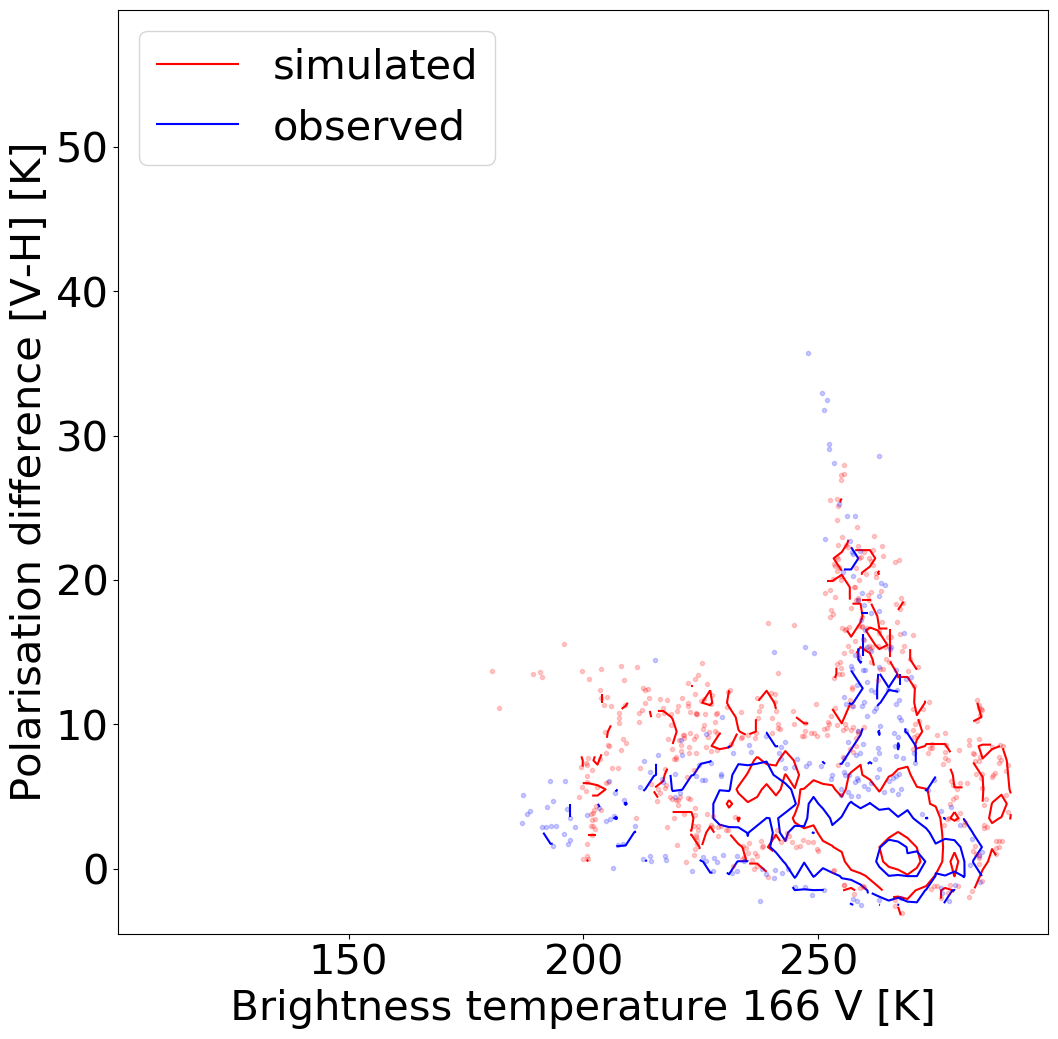
\includegraphics[height =35mm]{Figures/hist2d_gmi_45-60_land.png}
	\end{subfigure}
	\begin{subfigure}{.24\textwidth}
		\caption{Water}
		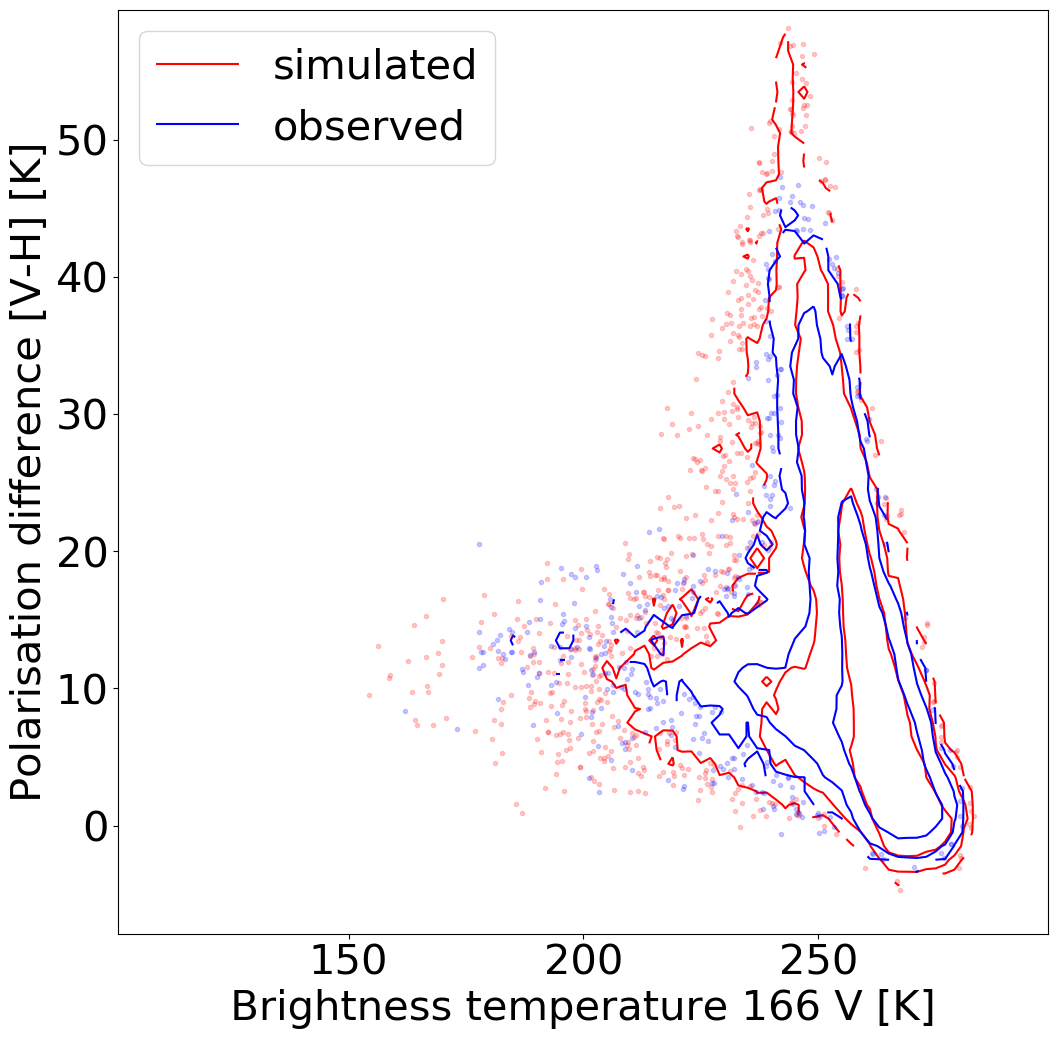
\includegraphics[height = 35mm]{Figures/hist2d_gmi_45-60_sea.png}
	\end{subfigure}
	\begin{subfigure}{.24\textwidth}
	\caption{Snow}
	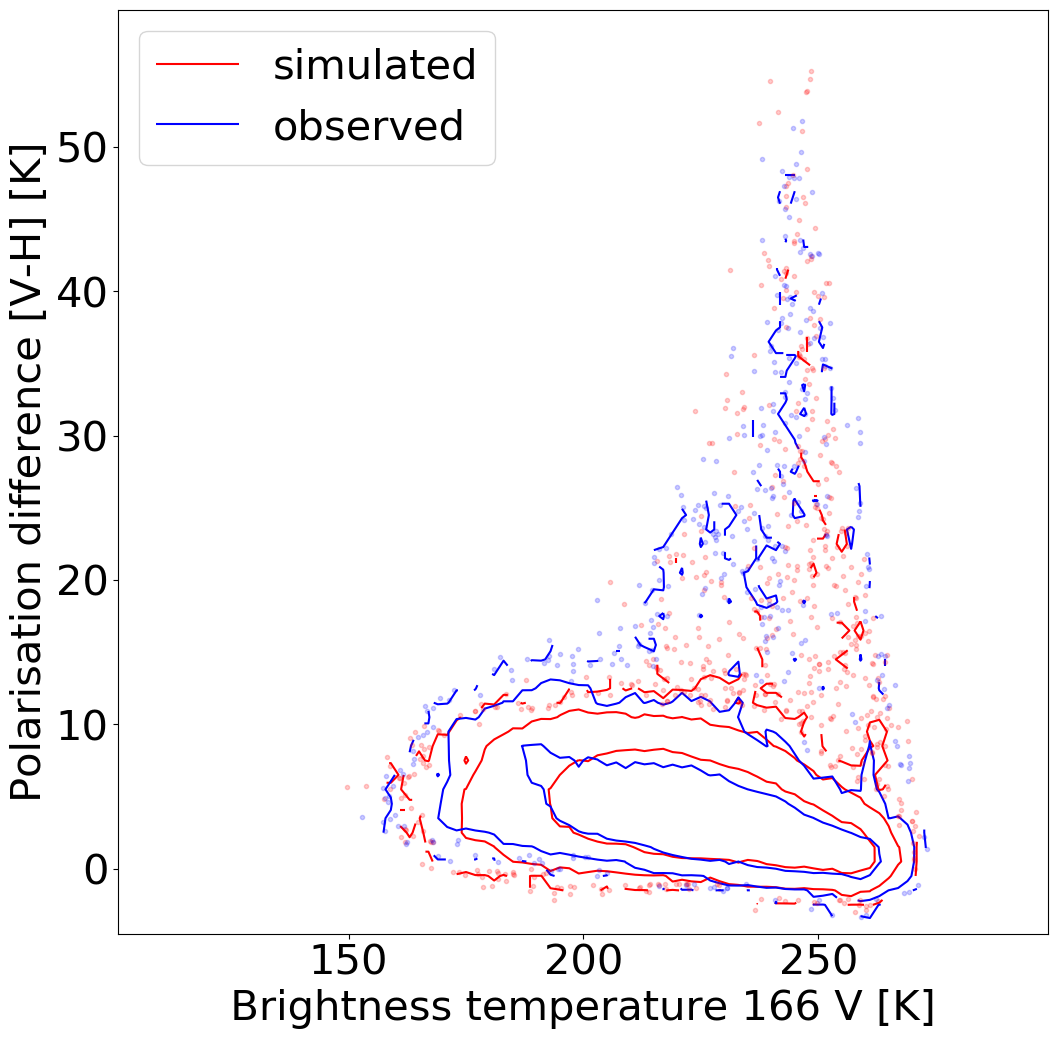
\includegraphics[height = 35mm]{Figures/hist2d_gmi_45-60_snow.png}
\end{subfigure}
\begin{subfigure}{.24\textwidth}
	\caption{ Sea-ice}
	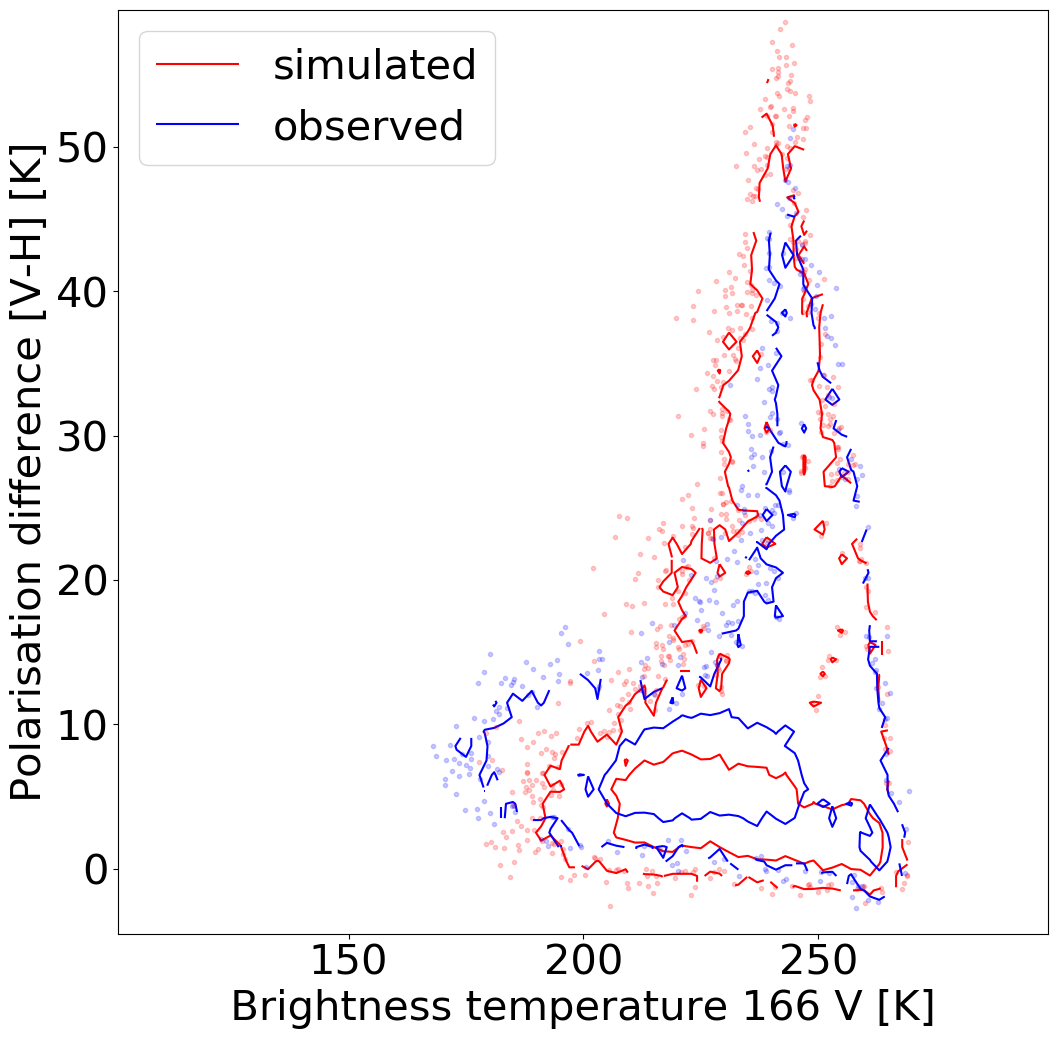
\includegraphics[height = 35mm]{Figures/hist2d_gmi_highlat_sea-ice.png}
\end{subfigure}
	\label{fig:histogram_2d}
	\caption{Two-dimensional PDFs for the TB and PD for GMI 166\,GHz frequency. Figures (a)-(d) are for land, water, snow and sea-ice surface types respectively.}
\end{figure*}

In order to verify that the data in the training database covers the actual measurement space, the measured and simulated TB from GMI are compared statistically. Figure~\ref{fig:histogram_2d} shows the polarisation difference (PD) and TB histograms from 166 GHz for different surface types. The PD is defined as difference between V and H polarisations. The effect of including particle orientation using the scheme of \citep{baralakas:intro:21} indeed looks promising to mimic the effect of hydrometeor interaction.
Over both sea-ice and snow, the PDs are mostly positive as a consequence of hydrometeor scattering, and the negative PDs arise from noise in clear-sky measurements. For all surface types, the variability of our simulations is higher than the GMI measurements, indicating that the simulations can cover the all possible range of conditions. This is important as we cannot expect the retrieval to provide a complete picture, if the training database covers the measurement range partially.



\subsubsection{Retrievals}

\begin{figure*}[t]
	\centering
	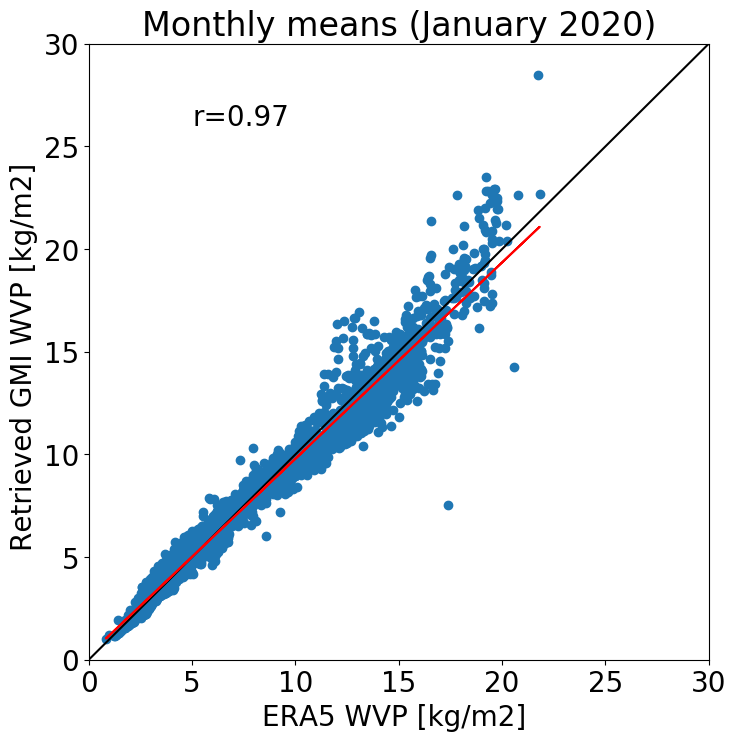
\includegraphics[height = 40mm]{Figures/WVP_scatter_monthlymean.png} 
	\label{fig:wvp_scatter}
	\caption{Scatterplot between monthly means derived from WVP retrieved from QRNN and ERA5. The data is for January 2020. The red line is the line of best fit, while the black indicates the perfect fit.}
\end{figure*}

The QRNN algorithm described in sec~\ref{sec:qrnn} is applied to TB from 166 \,GHz and 183\,GHz to retrieve the corresponding WVPs. A comparison of the monthly means for the retrieved WVP and ERA5 WVP is displayed in fig.~\ref{fig:wvp_scatter}. To enable comparison on common scales, both datasets were re-gridded to 2.5$^{\circ}$. The correlation between the monthly means between the two datasets is 0.97. 


\subsection{A: Retrievals}
\subsubsection{Work packages}

\todo{add a flowchart}

\subsubsection*{A1: Basic atmospheric scenarios}

As pointed out in \citet{eriksson:towar:20}: The input to the simulations can
be obtained from atmospheric models providing a sufficiently detailed
description of hydrometeors \citep[e.g.][]{wang2017statistical}. This approach
relies on that the model mimics reality with sufficient accuracy, as it
represents the a priori for the retrievals. Another option is to base the
simulations directly on observations as far as possible. In this study, we shall base the input to simulations through model observations. Over two sub-domains of Arctic, regional reanalyses performed with HARMONIE-AROME system at 2.5\,km resolution are available. This additional reanalyses available for European Arctic have improved parametrisations and extensive use of satellite data not previously used. Additionally, another option could be to use ICON model
(\url{www.mpimet.mpg.de/en/science/models}) that our colleagues in Hamburg have direct access to. 

\subsubsection*{A2 : Sea-ice emissivity}

0.5 page

	- Sea-ice Emissivity 
		- HR identification of sea-ice 	(info from Leif, figure?)
		- 1D VAR retrievals of sea-ice emissivity?  
	
\subsubsection*{A3 : Database creation}
	
This WP covers to launching and supervising the batch radiative transfer calculations (by ARTS).
Initially some time will be needed to implement the scripts needed for the basic calculations,
to add jobs to the calculation cluster and the post-processing needed. WP output is batches of
simulated radiances that are put into one or several retrieval databases.

\subsubsection*{A4 : Antenna pattern}

AMSR2 frequencies have different spatial resolutions. To generate the antenna pattern at a the desired frequency, a number of pencil beam radiative transfer calculations are performed to incorporate both along-track and across-track sampling. 

	

\subsubsection*{A5 : Retrieval setup}

The package for QRNN is already available as a part the Typhon software package \citep{lemke:2020:typho}. The implementation of the retrieval algorithm shall be relatively straightforward but the challenge would be to find the best performing neural-network architecture so as to achieve the best model performance. Besides, it would also be important to test the sensitivity of various auxiliary data to the retrieval performance. In order to run the retrievals, we shall make use of the Chalmers central computational cluster (C3SE).

\subsubsection*{A6 : WVP retrieval}

\subsubsection*{A7 : Liquid water content retrieval}


\subsection{B: Analysis and application}

In order to evaluate the quality of the retrievals, in this work package, we shall aim at reviewing the performance with other available products.

\subsubsection{Work packages}
\subsubsection*{Assessment with available products}



\subsubsection*{Applications}

\subsection{Risk Assessment}
0.5 page

\section{Collaborations}

In order to recieve feedback on the retrieval database, we would closely collaborate with group lead by Georg Heygster, University of Bremen to cover the analysis and validation aspects. Additionally, a contact with the group of Prof. Susanne Crewell would be also be useful for validation purposes. Their group is operating the MiRaC airborne sensor (a combined radar and radiometer) during polar flights (Mech et al., 2019).

ECMWF assimilation?

\section{Staff situation}
\label{sec:staff}
%
Inderpreet Kaur (IK) started as a postdoctoral researcher in the division during March 2020.  She is presently working with both millimetre (mm) and sub-millimetre (mm) data for retrieval of atmospheric ice, and is interested in machine learning techniques for retrieval applications. During the project period, she shall spend almost 100\,\% of her time the project. 

Patrick Eriksson (PE) is a professor, .... time contribution??

Luisa Ickes (LI) started as an assistant professor during Jan 2020, and  general field is atmospheric modelling and the special research interests are the Arctic region and clouds in general. She will provide expertise in cloud physics, both when generating training data and evaluating retrievals.

Leif Eriksson (LE) is group leader for the research group Radar Remote Sensing. His research is aimed at development of methods to make measurements of land and ocean with radar data. In this project, his expertise is sought on the use of synthetic aperture radar (SAR) observations to identify sea ice concentration.

\section{Satellite data}
%
All satellite data of concern will be publicly available, as coming from
operational weather sensors.

{\footnotesize
	\bibliography{j_abbr,refs_pe1,references}
}
\end{document}
